\section{Résultats}

\subsection{Tri du jeu de données}

Le jeu de données initial contient 175 799 SNPs.
\todo[color=blue!20]{À checker partout: loci ou SNPs? Si c'est juste une paire de bases dont tu parle, mieux vaut utiliser SNP, avec 'loci' on a tendance à penser que c'est une séquence entière.}
Pour le jeu de données utilisé au niveau de la sous-section \textit{Erythrodrosum}, 2 078 \textit{loci} ont été conservés pour les analyses, avec les seuils suivants :  fréquence des allèles rares $>$ 5\%, Phred $>$ 20, une distance de 10kb minimum entre deux \textit{loci} et 5\% des individus sans information maximum par \textit{locus}.
Pour le jeu de donnée sur le \clade{Hirsuta}, 1 851 \textit{loci} ont été conservés pour les analyses, avec les mêmes seuils.

Le changement de taille du jeu de donnée est du à un nombre plus petit d'individus dans le second cas, qui rend des \textit{loci} monomorphes. Le seuil le plus strict est le seuil sur les données manquantes par \textit{locus}, qui ne conserve que  respectivement 7.05\% et 7.07\% du jeu de donnée. 

\subsection{Sous-section \textit{Erythrodrosum}}

Dans un premier temps, le $F_{st}$ général entre les différents taxons de la sous-section \textit{Erythrodrosum} donne une valeur de 0.15.%, ce qui appuie l'hypothèse la présence d'une structure génétique. Cette structure était attendue étant donné qu'il s'agit de plusieurs espèces, mais pour autant il est important de remarquer que la valeur reste faible.
% Erythrodrosum
%            pop        Ind
% Total 0.1556567 -0.1016958
% pop   0.0000000 -0.3047961
%\todo[color=blue!20]{quid du Fis $<$0}

\begin{wrapfigure}{r}{0.30\textwidth}
	\vspace{-20pt}
	\begin{center}
	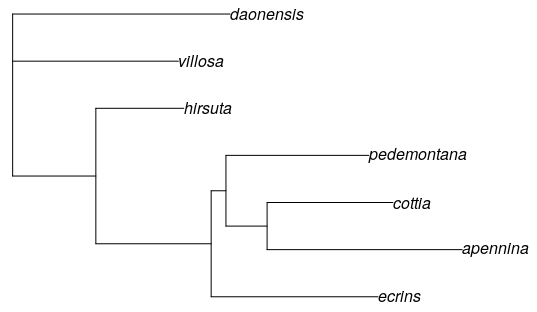
\includegraphics[width=0.29\textwidth]{fig/topologie.png}
	\end{center}
	\caption{\textbf{Topologie de la sous-section \textit{Erythrodrosum} obtenue par Neighbor-joining}, réalisé à partir de la matrice de distances $F_{st}$ par paires de populations.}
    \label{topologie}
\end{wrapfigure}

Les $F_{st}$ entre paires d'espèces sont également tous supérieurs à zero (valeurs comprises entre 0.093 et 0.214), et les relations phylogénétiques entre espèces obtenues par neigbhor-joining à partir de ces valeurs de $F_{st}$ rejoignent celles décrites précédemment (Figure \ref{topologie}).
\iffalse
\begin{wraptable}{r}{0.20\textwidth}
\vspace{-20pt}
\begin{tabular}{cc}\\\toprule  
K & BIC \\ \midrule
1 & 121.8305\\
2 & 120.3166\\
\textbf{3} & \textbf{119.9053}\\
4 & 120.8310\\
5 & 122.0690\\ \bottomrule
\end{tabular}
\label{BIC}
\vspace{-20pt}
\end{wraptable} \fi
Cette structure est par ailleurs confirmée par le clustering réalisé par adegenet sans \textit{a priori} de populations. Ainsi, le nombre K de clusters avec le critère d'information bayésien le plus faible est atteint pour K=3. La valeur de BIC la plus proche est celle de K=2, avec une différence de 0.41 (K=3 119.90; K=2 120.31). La valeur de K=4 présente également un BIC très proche (K=4 120.83). Pour la valeur de K=3, les groupes sont corrélés à la géographie, avec un \clade{est-alpin} composé de \textit{P. daonensis} et \textit{P. villosa}, un clade composé de l'espèce \textit{P. hirsuta} et enfin \textit{P. pedemontana s.l.}.

% K=1      K=2      K=3      K=4      K=5      K=6      K=7      K=8      K=9     K=10     K=11     K=12     K=13     K=14     K=15     K=16     K=17     K=18     K=19     K=20 
% 121.8305 120.3166 119.9053 120.8310 122.0690 123.3748 124.7359 125.7829 126.8601 127.9004 128.7918 129.0472 129.3280 129.0943 128.6408 127.7302 125.9209 123.1317 117.1152 104.5158 
%BIC
\begin{wrapfigure}{r}{0.5\textwidth}
	\vspace{-20pt}
	\begin{center}
    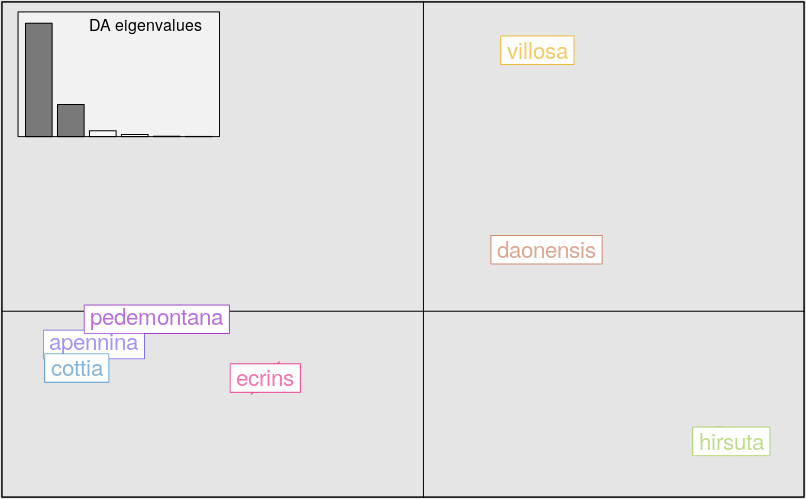
\includegraphics[width=0.49\textwidth]{fig/DAPC.png}
    \caption{\textbf{Analyse en composante principale discriminante de la sous-section \textit{Erythrodrosum} Pax.} Les groupes à priori sont les populations échantillonnées.}
    \label{dapc}
    \end{center}
    \vspace{-20pt}
\end{wrapfigure}

Ce clustering est plus facilement visualisable sous la forme d'une analyse en composante principale discriminante comme dans la figure \ref{dapc}. Les deux premières composantes montrent ce clustering avec quelques précisions de plus. Ainsi, les individus de \textit{P. pedemontana s.l.}. sont plus proches que ceux du \clade{est-alpin}. Cependant, la population des Écrins n'est pas aussi groupée que le reste des populations composant \textit{P. pedemontana s.l.}, et s'en éloigne vers \textit{P. hirsuta}.

\subsection{Clade `Hirsuta'}

La structuration du \clade{Hirsuta} pour différentes valeurs de K permet de voir différentes informations (figure \ref{structure}). Pour K=2, une séparation est déjà nette entre deux clades, conformément aux résultats précédents, entre \textit{P. pedemontana s.l.} et \textit{P. hirsuta}. Cette séparation présente néanmoins une légère trace d'admixture entre les individus des Écrins et \textit{P. hirsuta}. L'individu de \textit{P. hirsuta} présentant un peu d'admixture a été échantillonné en Belledonne, un massif proche des Écrins (figure \ref{carte}).

\begin{wrapfigure}{r}{0.50\textwidth}
	\vspace{-40pt}
	\begin{center}
	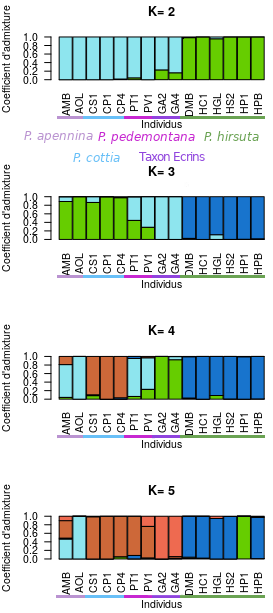
\includegraphics[width=0.49\textwidth]{fig/structure_hirsuta.png}
	\end{center}
	\caption{\textbf{Structuration du \clade{Hirsuta} par sNMF.} Les K choisis vont de 2 à 5, avec 20 répétition par K et choix du meilleur run sur critère de cross-entropy.}
    \label{structure}
    \vspace{-20pt}
\end{wrapfigure}


Pour K=3, les individus des Écrins sont isolés et une admixture entre ces individus et les autres individus de \textit{P. pedemontana s.l.}. Cette structure retrouvée ici reflète ce qui étais observé sur la DAPC, où les individus des Écrins se regroupaient avec \textit{P. pedemontana s.l.} tout en étant excentré.

Pour K=4, \textit{P. pedemontana s.l.} se retrouve éclaté avec les différentes populations échantillonnées dans les divers massifs. Cependant, les deux espèces \textit{P. apennina} et \textit{P. cottia} sont toujours regroupées, même si cet ensemble n'est pas retrouvé pour K=5. C'est alors \textit{P. hirsuta} qui se retrouve scindé en deux avec d'un côté l'individu des Pyrénées et de l'autre l'ensemble des individus. Ici la structure de \textit{P. pedemontana s.l.} est donc plus ambigue, même si les individus des Écrins sont toujours isolés. Il est donc remarquable qu'au delà de K=3, aucune structure regroupant durablement des individus est observable.

%Pour les analyses sur DIYABC, aucun scénario proposé ne permet de simuler un jeu de donnée proche des données réelles. Le scénario observé le plus proche des données réelles étais celui d'un polytomie où coalescent tout les taxons assigné à l'espèce \textit{P. pedemontana}), puis un événement plus ancien de coalescence avec \textit{P. hirsuta}. Ne pouvant conclure si cette polytomie est réelle ou alors un artefact issu d'un manque de résolution (soft poolytomie), les analyses n'ont pas été plus loin avec cette outil et aucun résultat ne peut être présenté.

\subsection{Hypothèse d'admixture}

Le test d'admixture entre les différentes populations de \textit{P. pedemontana s.l.} et \textit{P. hirsuta}, avec \textit{P. daonensis} en outgroup confirment l'admixture entre le taxon des Écrins et \textit{P. hirsuta} \ref{ABBA}. En effet, le D estimé est supérieur à 0 avec une moyenne de 0.102. A contrario, le test ne permet pas d'estimer un D différent de 0 pour les autres populations, ce qui reflète les observations précédentes en sNMF.

Cependant, il est important de noter que ce test ne permet pas d'estimer quelle population de \textit{P. pedemontana s.l.} s'est admixté avec \textit{P. hirsuta}, vu que le résultat est positif quelque soit la population sélectionnée en P1.

\begin{table}[!h]
\begin{tabular}{ccccccc}\\\toprule  
P1 & P2 & P3 & Outgroup & D & p-valeur \\ \midrule
\textit{P. pedemontana} & \textit{P. apennina} & \textit{P. hirsuta} & \textit{P. daonensis} & -0.027 & 0.212 \\
\textit{P. pedemontana} & \textit{P. cottia} & \textit{P. hirsuta} & \textit{P. daonensis} & -0.033 & 0.0772 \\ \midrule
\textit{P. pedemontana} & Taxon des Écrins & \textit{P. hirsuta} & \textit{P. daonensis} & \textbf{0.082} & \textbf{5.761.10$^{-5}$} \\
\textit{P. apennina} & Taxon des Écrins & \textit{P. hirsuta} & \textit{P. daonensis} & \textbf{0.109} & \textbf{6.465.10$^{-7}$} \\
\textit{P. cottia} & Taxon des Écrins & \textit{P. hirsuta} & \textit{P. daonensis} & \textbf{0.116} & \textbf{1.237.10$^{-8}$} \\ \bottomrule
\end{tabular}
\caption{\textbf{Test d'admixture par ABBA-BABA}. La p-valeur est estimée à partir d'un bootstrap sur les \textit{loci}. Un D supérieur à 0 indique une admixture entre P2 et P3.}
\label{ABBA}
\end{table}

% Ce résultat permet par contre de proposer deux hypothèses : la proximité génétique entre ces trois espèces ou alors une admixture passée avant séparation de ces populations sur des massifs isolés.
